\chapter{Eksperymenty} \label{ch:experiments}

\section{Parametry systemu testowego}

Testy przeprowadzane były na systemie
\begin{itemize}
	\item \textbf{OS}: Ubuntu 15.10,
    \item \textbf{Wersja kernela}: 4.2.0.16-generic,
    \item \textbf{Dysk}: Seagate ST1000DM003 1TB sATA III 64MB
    \begin{itemize}
    	\item \textbf{Format}: 3,5 cali,
        \item \textbf{Pojemność}: 1000 GB,
        \item \textbf{Interfejs}: Serial ATA III,
        \item \textbf{Prędkość obrotowa}: 7200 rpm,
        \item \textbf{Pamięć cache}: 64 MB,
        \item \textbf{Technologia przechowywania}: HDD,
        \item \textbf{Średnie opóźnienie}: 4,16 ms
    \end{itemize}
\end{itemize}
\section{Wyniki}

Poniżej przedstawiono otrzymane wyniki dla limitów szybkości transferu danych: 
\begin{itemize}
	\item bez limitów,
    \item 100 MB/s,
    \item 60 MB/s,
	\item 20 MB/s, 
    \item 5MB/s.
\end{itemize}

Dla każdej obliczono
\begin{itemize}
	\item przepustowość pasma,
    \item ilość operacji na sekundę,
    \item opóźnienie
\end{itemize}

\begin{figure}[h]
	\centering
	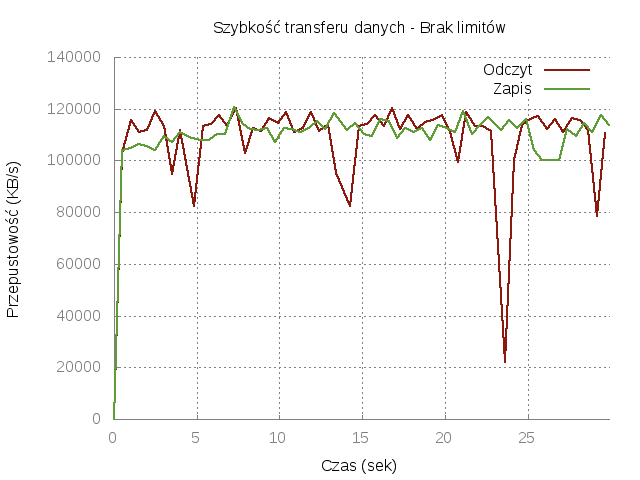
\includegraphics[scale=0.9]{results/Unlimited_bw.png}
		\caption{Brak limitów, przepustowość}
    \label{fig:unlimited-bw}
\end{figure}
\begin{figure}[h]
	\centering
	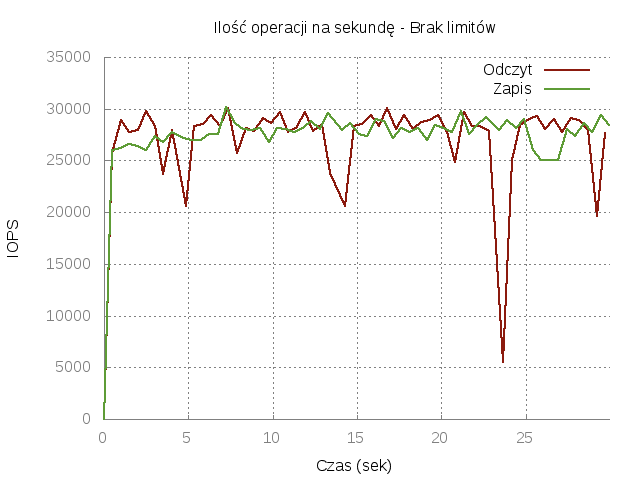
\includegraphics[scale=0.9]{results/Unlimited_iops.png}
		\caption{Brak limitów, ilość operacji na sekundę}
    \label{fig:unlimited-iops}
\end{figure}
\begin{figure}[h]
	\centering
	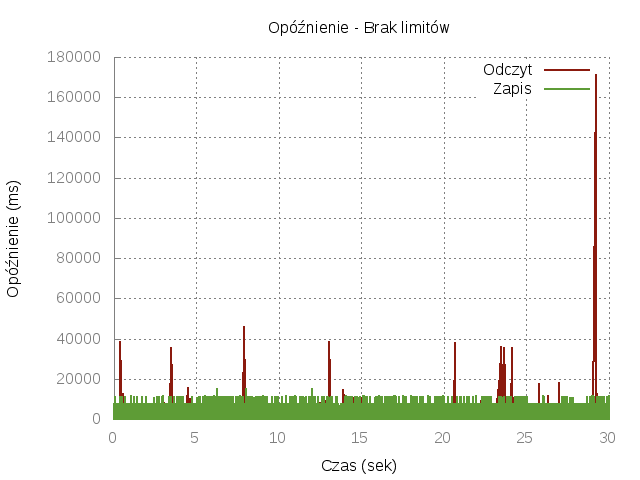
\includegraphics[scale=0.9]{results/Unlimited_lat.png}
		\caption{Brak limitów, opóźnienie}
    \label{fig:unlimited-lat}
\end{figure}

\begin{figure}[h]
	\centering
	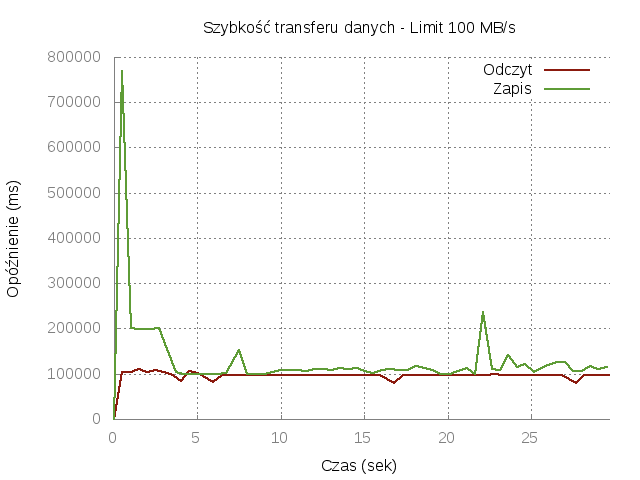
\includegraphics[scale=0.9]{results/100_bw.png}
		\caption{100 MB/s, przepustowość}
    \label{fig:100-bw}
\end{figure}
\begin{figure}[h]
	\centering
	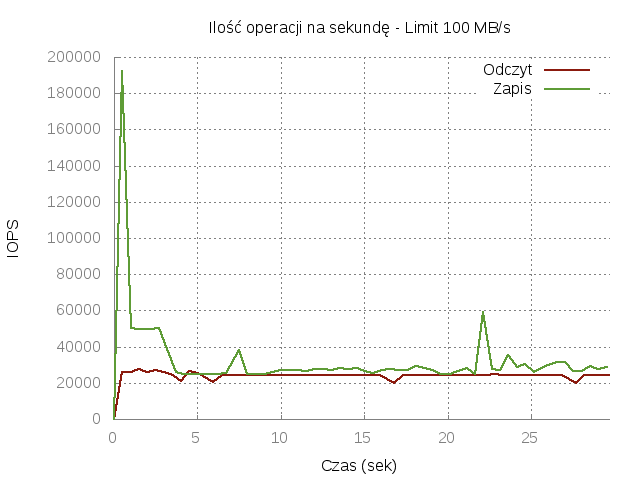
\includegraphics[scale=0.9]{results/100_iops.png}
		\caption{100 MB/s, ilość operacji na sekundę}
    \label{fig:100-iops}
\end{figure}
\begin{figure}[h]
	\centering
	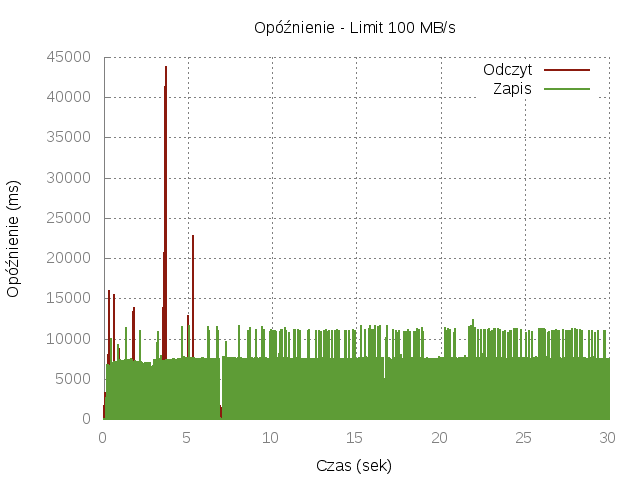
\includegraphics[scale=0.9]{results/100_lat.png}
		\caption{100 MB/s, opóźnienie}
    \label{fig:100-lat}
\end{figure}

\begin{figure}[h]
	\centering
	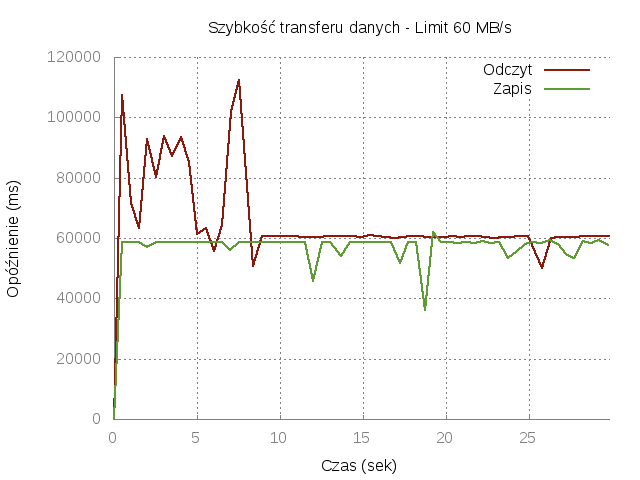
\includegraphics[scale=0.9]{results/60_bw.png}
		\caption{60 MB/s, przepustowość}
    \label{fig:60-bw}
\end{figure}
\begin{figure}[h]
	\centering
	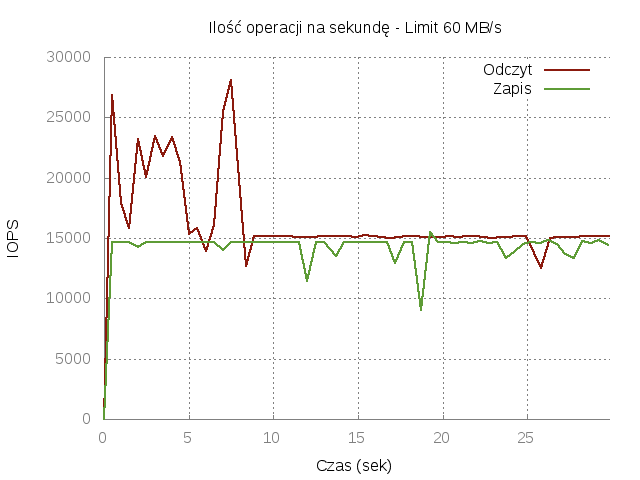
\includegraphics[scale=0.9]{results/60_iops.png}
		\caption{60 MB/s, ilość operacji na sekundę}
    \label{fig:60-iops}
\end{figure}
\begin{figure}[h]
	\centering
	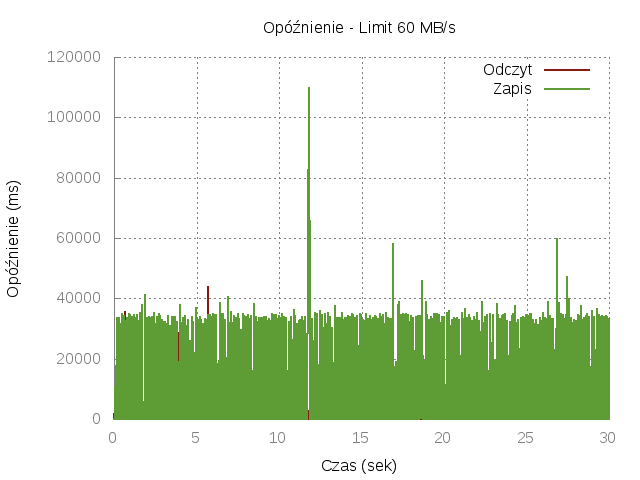
\includegraphics[scale=0.9]{results/60_lat.png}
		\caption{60 MB/s, opóźnienie}
    \label{fig:60-lat}
\end{figure}

\begin{figure}[h]
	\centering
	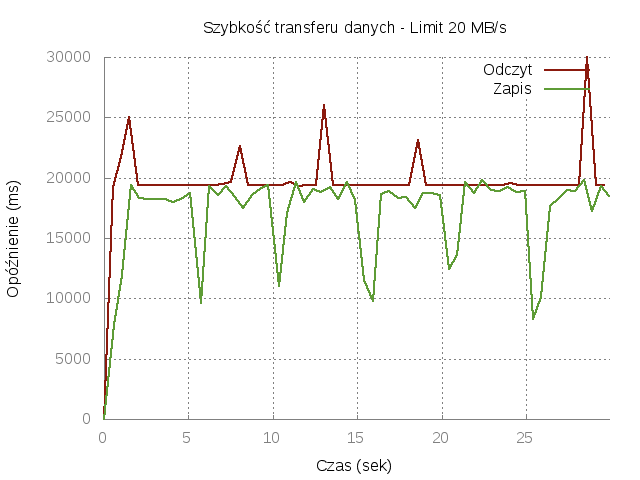
\includegraphics[scale=0.9]{results/20_bw.png}
		\caption{20 MB/s, przepustowość}
    \label{fig:20-bw}
\end{figure}
\begin{figure}[h]
	\centering
	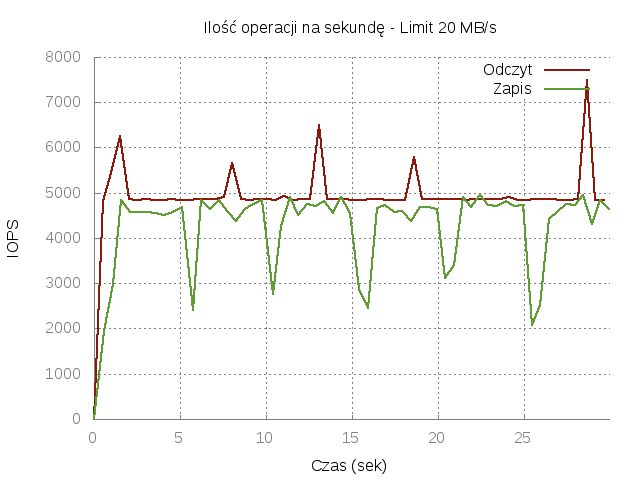
\includegraphics[scale=0.9]{results/20_iops.png}
		\caption{20 MB/s, ilość operacji na sekundę}
    \label{fig:20-iops}
\end{figure}
\begin{figure}[h]
	\centering
	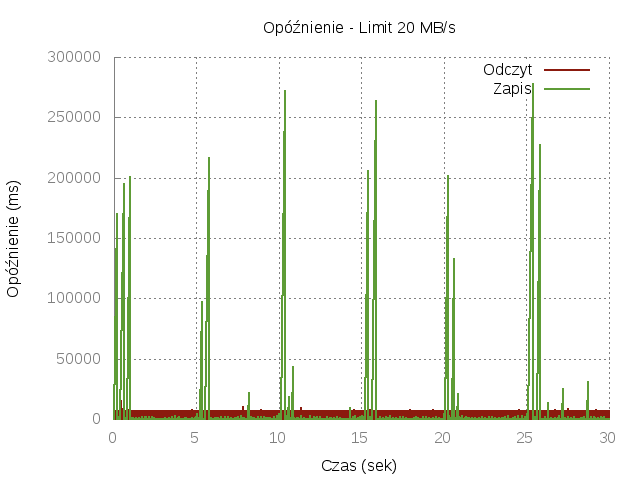
\includegraphics[scale=0.9]{results/20_lat.png}
		\caption{20 MB/s, opóźnienie}
    \label{fig:20-lat}
\end{figure}

\begin{figure}[h]
	\centering
	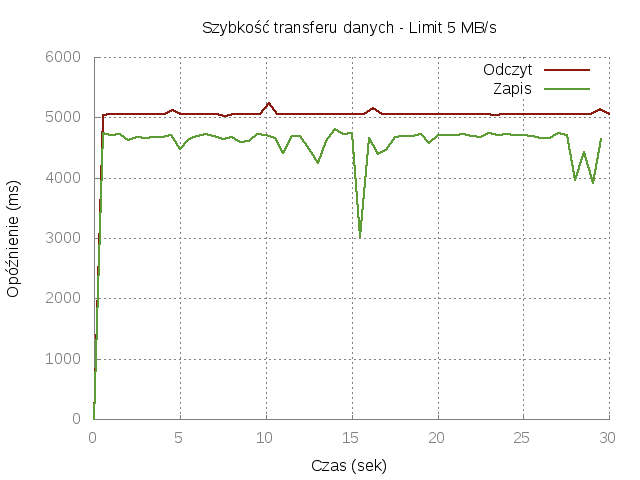
\includegraphics[scale=0.9]{results/5_bw.png}
		\caption{5 MB/s, przepustowość}
    \label{fig:5-bw}
\end{figure}
\begin{figure}[h]
	\centering
	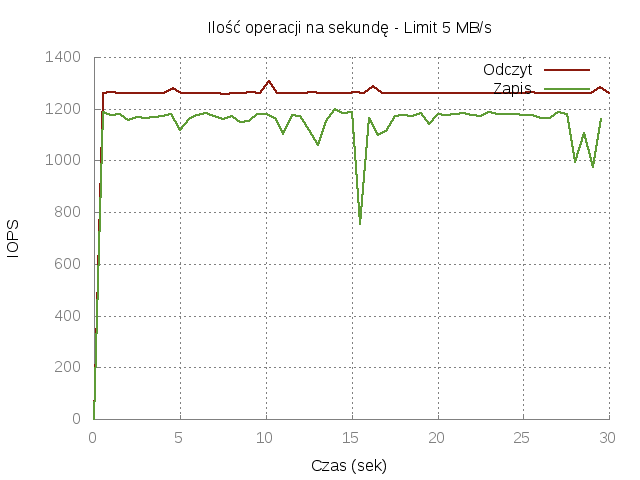
\includegraphics[scale=0.9]{results/5_iops.png}
		\caption{5 MB/s, ilość operacji na sekundę}
    \label{fig:5-iops}
\end{figure}
\begin{figure}[h]
	\centering
	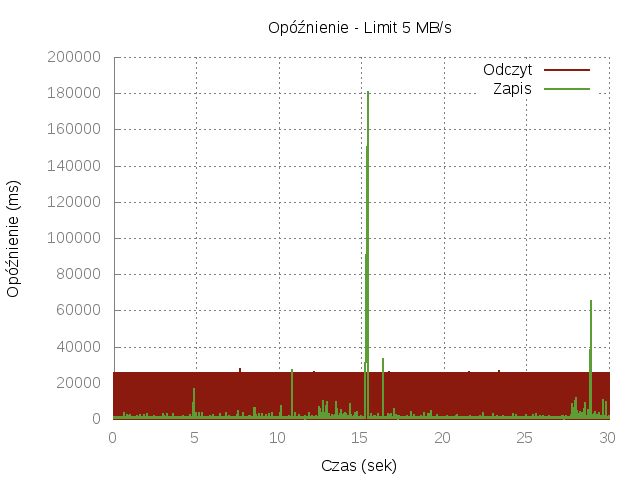
\includegraphics[scale=0.9]{results/5_lat.png}
		\caption{5 MB/s, opóźnienie}
    \label{fig:5-lat}
\end{figure}

\clearpage
\newpage
\section{Analiza wyników}
\subsection{Bez limitów}
Jak widać na wykresie \ref{fig:unlimited-bw}
nieograniczona szybkość transferu danych przyjmuje wartości z dużego zakresu. Dla operacji odczytu
waha się od \textbf{21933 Kb/s} do \textbf{120320 KB/s}, a dla zapisu od
\textbf{100000 KB/s} do \textbf{118400 KB/s}.

Ilość operacji na sekundę (IOPS, wykres \ref{fig:unlimited-iops}) jest powiązana bezpośrednio z szybkością transferu danych, dlatego
przebieg wykresu wygląda podobnie. Dla odczytu wartości wahają się
od \textbf{5483 IOPS} do \textbf{29696 IOPS}, a dla zapisu od \textbf{25000 IOPS}
do \textbf{29761 IOPS}.

Opóźnienie (wykres \ref{fig:unlimited-lat})
pokazują czas potrzebny na wykonanie operacji I/O. Wyraźnie widać, że
- dla odczytu - w okolicach 24 i 29 sekundy skoki w opóźnieniu opdowiadają
spadkom w szybkości transferu danych. Im dłuzszy czas potrzebny na przetworzenie
zlecenia operacji I/O, tym wolniejsza szybkość.

Na podstawie tych wyników można
zauważyć, że podczas przeprowadzania testów działają inne procesy, które
używają zasoby I/O, co powoduje spadki w szybkości transferu.

\subsection{100 MB/s}

Pierwszym z przeprowadzonych testów było ustawienie limitu szybkości zapisu i odczytu
na 100 Mb/s. Jak widać na wykresie \ref{fig:100-bw} i \ref{fig:100-iops}
podczas pierwszych 6 sekund
szybkość była niestabilna i przekroczyła narzucony limit dwukrotnie. Następnie, do końca testu,
utrzymywała się stabilnie poniżej 100 Mb/s a dwukrotnie spadła w okolice 80 Mb/s
(w 16 i 28 sekundzie). 

Początkową niestabilność można wytłumaczyć opóźnieniem (wykres \ref{fig:100-lat})
, które w pierwszych 6 sekundach miało niejednostajne wartości, różniące się nawet o
43 ms. Mimo tych nieregularności, szybkość transferu nigdy nie przekroczyła progu 111000 KB/s , co mieści się w 11\% narzuconego limitu. 

Dwa spadki w 16 i 28 sekundzie nie zależą od opóźnienia, a wywołane mogą być przez
chwilowy brak dostępnej szybkości. Jako, że nie przekraczają one limitu, nie stanowi to problemu
i system zadziałał prawidłowo.

Dla operacji zapisu szybkość transferu ustabilizowała sie wczesniej, koło 4 sekundy. Następnie utrzymywała się w okolicach limitu, poza dwoma momentami
(7 i 22 sekunda) gdzie wzrosła na chwilę nawet ponad 200 MB/s. Opóźnienia  utrzymywały się w okolicy 9 ms czasami zwiększając
się do 11ms.

\section{60 MB/s}

Dla odczytu limitowanego 60 MB/s szybkość stabilizowała się dłużej niż w przypadku 100 MB/s
- w okolicach 9 sekundy (wykres \ref{fig:60-bw} i \ref{fig:60-iops}).
Nastepnie wykorzystywana była przepustowość zgodna z założeniami, poza jednym spadkiem w
okolicach 26 sekundy. Stabilizacja szybkości jest również widoczna na wykresie \ref{fig:60-lat}, a spadek został spowodowany innymi czynnikami.

Wykres zapisu przebiega bardziej
chaotycznie. Od samego początku trzyma się ustalonych limitów, tylko raz osiągając
większą szybkość (odchył o 4\%) w 19 sekundzie. Wszystkie spadki spowodowane są opóźnieniem
dysku, co można zaobserwować na wykresie \ref{fig:60-lat}.

\section{20 MB/s}

Przy limicie ustawionym na 20 MB/s dla szybkości transferu danych podczas odczytu zaobserwowano największe odchyły od oczekiwanych wartości
(wykres \ref{fig:20-bw} i \ref{fig:20-iops}).
Przepustowość osiąga szybkości większe niż limit w okolicach 1, 7, 19, 29 sekundy.
Największy skok (w 29 sekundzie) osiąga 30 MB/s co stanowi 50\% limitu.

Skoki te są chwilowe i trwają krócej niż jedną sekundę a w pozostałych przypadkach
operacje są limitowane poprawnie. 

Opóźnienie (wykres \ref{fig:20-lat}) utrzymuje stałą wartość w okolicach 6 ms
z nielicznymi skokami do 8-10 ms oraz 14 ms na początku testu.

Wartości szybkości transferu danych, mimo iż nigdy nie przekroczyły limitu 20 MB/s  ciągle się
zmieniały. Zanotowano regularne spadki co około 5 sekund (6, 11, 16, 21, 26 sekunda)
w okolice 8200-10000 KB/s.

Spadki te łatwo wytłumaczyć obserwując opóźnienia (wykres \ref{fig:20-lat}).
Każdemu spadkowi odpowiada znaczny skok opóźnienia w okolice 200-260 ms.

\section{5 MB/s}

Dla najniższego z testowanych limitów - 5 MB/s szybkości transferu danych 
są najbardzie stabilne z wszystkich testowanych przypadków. Dla odczytu
(wykres \ref{fig:5-bw} i \ref{fig:5-iops}) w pierwszej sekundzie transfer osiąga szybkość w okolicach
5 MB/s i utrzymuje ją w całym czasie trwania testu z nieznacznymi skokami w
9, 10, 16 i 29 sekundzie. Skoki te nie przekraczają 5.3 MB/s, co stanowi 6\%
limitu.

Opóźnienie przyjmuje stała wartość 25 ms (wykres \ref{fig:5-lat}) z nielicznymi
małymi skokami.

Operacje zapisu również
nie przekraczają limitu 5 MB/s ale, tak samo jak w poprzednich przypadkach, pojawiają się spadki
szybkości transferu danych. Największy z nich ma miejsce w 16 sekundzie i osiąga wartość 3 MB/s.
Spadki te można zauważyć również badając opóźnienie (wykres \ref{fig:5-lat}).

